\documentclass[a4paper, 12pt]{article}

\usepackage[top=2cm, bottom=2cm, left=2.5cm, right=2.5cm]{geometry}
\usepackage[utf8]{inputenc}
\usepackage{array}
\usepackage{graphicx}
\usepackage{listings}
\usepackage{caption}
\usepackage[labelfont=bf]{caption}

\captionsetup[lstlistings]{position=bottom}
\graphicspath{{img/}}

\begin{document}
\lstset{language=SQL}
\begin{flushleft}
\includegraphics{logo}\\
\textbf{UNIVERSIDADE TECNOLÓGICA FEDERAL DO PARANÁ | UTFPR} \\
\textbf{ALUNO:} Ricardo Medeiros da Costa Junior   \textbf{RA:} a1598996 \\
\textbf{DISCIPLINA:} Banco de Dados para Biologia \\
\textbf{ATIVIDADE:} Sistema de Recomendações | Tarefa 2 

\section{Persistência dos dados}
Foram persistidos todos os nós e relações no banco de dados, exatamente como foi orientado no documento da ativida, utilizando a linguagem \emph{Cypher}. Após realizado todas inserções, o banco de dados completo é semelhante ao da Figura 1.
\begin{figure}[hb]
  \centering
  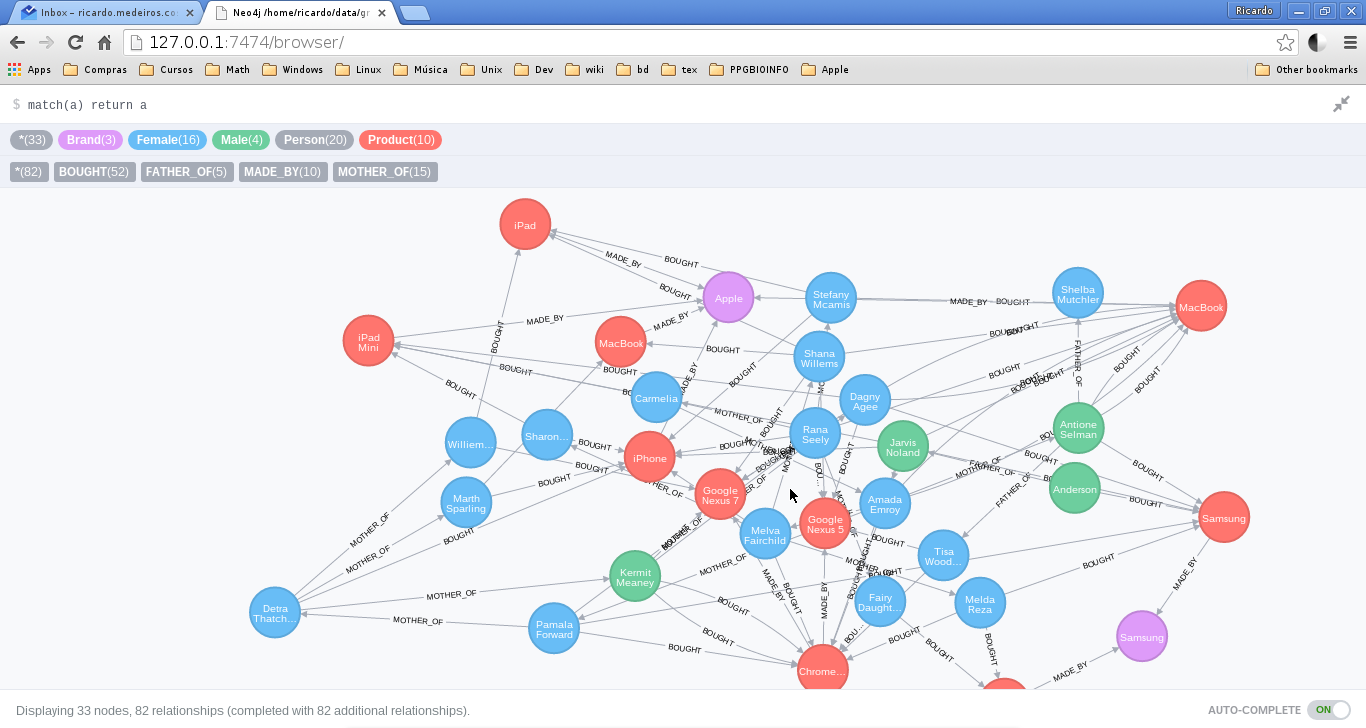
\includegraphics[width=7in]{1}
  \caption[1 - Banco de dados criado]{\textbf{Banco de dados criado}}
\end{figure} \\
O banco criado possui 33 nós e 82 relações.

\section{Recomendações baseada em compras de produtos}
A lógica para essa consulta foi a seguinte: Relaciona com essa pessoa, produtos comprados por outras pessoas que compraram produtos iguais ao que a pessoa comprou. No entanto, são relacionados apenas produtos que a pessoa não comprou. O código da consulta \emph{Cypher} torna mais claro esse conceito. \\

\begin{lstlisting}[frame=single]
match (person:Person)-[:BOUGHT]->(product:Product)
 <-[:BOUGHT]-(anotherPerson:Person)
  -[:BOUGHT]->(anotherProduct:Product)
where not (person)-[:BOUGHT]->(anotherProduct)
return person.name, collect(distinct anotherProduct.name)
order by person.name
\end{lstlisting}
%\captionof{lstlistings}{}%

\end{document}
